\chapter{Background}
This chapter introduces the concepts used in the rest of the report, reviews the literature on audio-driven talking-head generation and similar applications, and identifies the gap this project addresses.

\section{Preliminaries}
In this section, we provide the background knowledge needed to understand the rest of our report.\\

\noindent
\textbf{Audio-driven talking-head generation:} Generating video of a face whose lip movements follow a given speech signal.

\noindent
\textbf{Person-specific and person-generic models:} A person-specific model is trained for one face and must be retrained for each new person; a person-generic model works on any face without retraining, usually at a higher computational cost.

\noindent
\textbf{U-Net inpainting:} An encoder--decoder network with skip connections. In SyncTalk\_2D it receives a video frame with the mouth region blacked out and ``paints'' the mouth back in, conditioned on the audio.

\noindent
\textbf{Audio features:} Speech is converted into a sequence of numerical features before it reaches the network, for example a mel spectrogram, the output of an audio--visual encoder, or the internal representation of a self-supervised speech model.

\noindent
\textbf{Self-supervised speech encoders (wav2vec~2.0, XLS-R):} Models pre-trained on large amounts of unlabelled speech \cite{baevski2020wav2vec2}. XLS-R \cite{babu2022xlsr} is pre-trained on 128 languages, including Bangla, and its intermediate layers capture phonetic content.

\noindent
\textbf{SyncNet and LSE:} SyncNet \cite{chung2016outoftime} is a network that judges whether a mouth and an audio clip are in sync. From it come the two standard lip-sync metrics: LSE-D (lip-sync error distance; lower is better) and LSE-C (lip-sync error confidence; higher is better).

\noindent
\textbf{Phoneme and viseme:} A phoneme is a distinct speech sound; a viseme is a visually distinct mouth shape. Several phonemes can share a viseme, so a phoneme-to-viseme mapping is many-to-one.

\noindent
\textbf{Leakage:} Mouth motion in a generated video that comes from the input video rather than from the audio. A model that leaks can look well synchronised while ignoring the speech. It is measured by driving the model with silent audio and counting the frames in which the mouth is open \cite{bigata2025keysync}.

\noindent
\textbf{Speech-to-speech conversational model:} A large language model that takes speech in and produces speech out directly, instead of passing through separate speech-recognition and speech-synthesis stages.

\noindent
\textbf{Voice Activity Detection (VAD):} Detecting when a person is speaking, used to decide when the user has finished their turn.

\noindent
\textbf{Real-Time Communication (RTC):} Low-latency streaming of audio and video between browser and server, provided here by LiveKit over WebRTC.

\noindent
\textbf{Neural Radiance Fields (NeRF) and 3D Gaussian Splatting (3DGS):} 3D scene representations used by several recent talking-head systems. NeRF represents the head as a continuous neural field; 3DGS represents it as many small 3D Gaussian ``splats'', which render much faster.


\section{Literature Review}

Speech-driven talking-head synthesis has developed in stages: from 2D image-based animation, to 3D neural representations, to fast Gaussian-Splatting rendering. Each stage addressed the weaknesses of the one before and introduced new trade-offs.\\

\noindent
\textbf{2D animation.} Early work animated a single static image. MakeItTalk \cite{DBLP:journals/corr/abs-2004-12992} separated the speech content from the speaker's identity to drive facial landmarks and head motion from one image, and produced convincing lip-sync and expression control. As a 2D method it did not represent 3D geometry, so head rotation and depth-dependent motion were not consistent.\\

\noindent
\textbf{Neural radiance fields.} To obtain 3D consistency, later work conditioned Neural Radiance Fields on audio. AD-NeRF \cite{DBLP:journals/corr/abs-2103-11078} was the first to do so, producing 3D-consistent, high-fidelity talking faces and upper bodies from new viewpoints. It tied facial motion closely to the radiance field, however, which gave little control over individual facial attributes. DFA-NeRF \cite{DBLP:journals/corr/abs-2201-00791} disentangled lip motion from head pose and blinking for more personalised and controllable generation. NeRF-based methods nonetheless remained slow to train and to render, which made real-time use impractical.\\

\noindent
\textbf{Synchronisation.} SyncTalk \cite{peng2024synctalkdevilsynchronizationtalking} made synchronisation the central problem, aligning audio, lip movement, facial expression and head pose through a face-sync controller and stabilising mechanisms. It clearly improved temporal coherence and realism over earlier NeRF models, but kept NeRF's computational cost.\\

\noindent
\textbf{Gaussian Splatting.} Recent work replaced NeRF with explicit 3D Gaussian Splatting to remove the computational bottleneck. GaussianTalker \cite{cho2024gaussiantalkerrealtimehighfidelitytalking} rendered audio-driven 3D Gaussian talking heads in real time with high visual quality. TalkingGaussian \cite{li2024talkinggaussianstructurepersistent3dtalking} kept the static facial structure separate from the audio-driven deformation, reducing distortion in highly dynamic regions such as the mouth. GaussianSpeech \cite{aneja2024gaussianspeechaudiodrivengaussianavatars} added finer explicit modelling of the teeth and inner mouth, and NeRFFaceSpeech \cite{kim2024nerffacespeechoneshotaudiodriven3d} generated 3D-aware animation from a single image using generative priors. InsTaG \cite{li2025instaglearningpersonalized3d} combined Gaussian Splatting with a universal motion field learned in pre-training, so that a new person can be learned from a few seconds of video.\\

\noindent
\textbf{2D lip-synchronisation.} In parallel, 2D methods edit only the mouth region of an existing video. Wav2Lip \cite{prajwal2020wav2lip} trained a generator against a pre-trained SyncNet ``lip-sync expert'' \cite{chung2016outoftime} and became the most widely used baseline. IP-LAP \cite{zhong2023iplap} adds landmark and appearance priors to preserve identity, and MuseTalk \cite{zhang2024musetalk} and LatentSync \cite{li2024latentsync} generate the mouth in the latent space of an image or diffusion model. SyncTalk\_2D \cite{synctalk2d} is a lightweight person-specific 2D U-Net designed for real-time use, and is the model this project builds on.\\

\noindent
\textbf{Leakage.} Because 2D methods see the rest of the face, they can learn to copy the mouth from the input video instead of generating it from the audio. LatentSync \cite{li2024latentsync} describes this as a shortcut that its training has to counter, and KeySync \cite{bigata2025keysync} proposed a masking strategy against it together with a leakage measure, LipLeak, which drives the model with silent audio. We use the same silent-audio test and extend it in Section~\ref{sec:leakage}.\\

\noindent
\textbf{The gap.} All of these systems are built and tested on high-resource languages, chiefly English, and give little attention to the phonetic and prosodic properties of low-resource languages such as Bangla. The most visually capable methods also need GPUs far beyond consumer hardware, and few report whether the mouth stays still in silence. Our work focuses on a Bangla talking head that runs in real time on a laptop, with its audio dependence verified directly.\\


\subsection{Similar Applications}
\begin{enumerate}
  \renewcommand{\labelenumi}{(\roman{enumi})}

\item
\textbf{Tavus and similar commercial platforms (2024--2025) : }Tavus generates personalised AI-driven talking avatars for sales and marketing, and platforms such as HeyGen offer real-time conversational avatars with voices in many languages, including Bangla. These systems are proprietary, depend on large datasets and cloud-scale compute, are paid per use, and publish no evaluation of how well their lips follow Bangla speech. Our system is open, targets Bangla specifically, measures its Bangla lip movement, and runs its avatar locally on consumer hardware.\\

\begin{figure}[H]
    \centering
    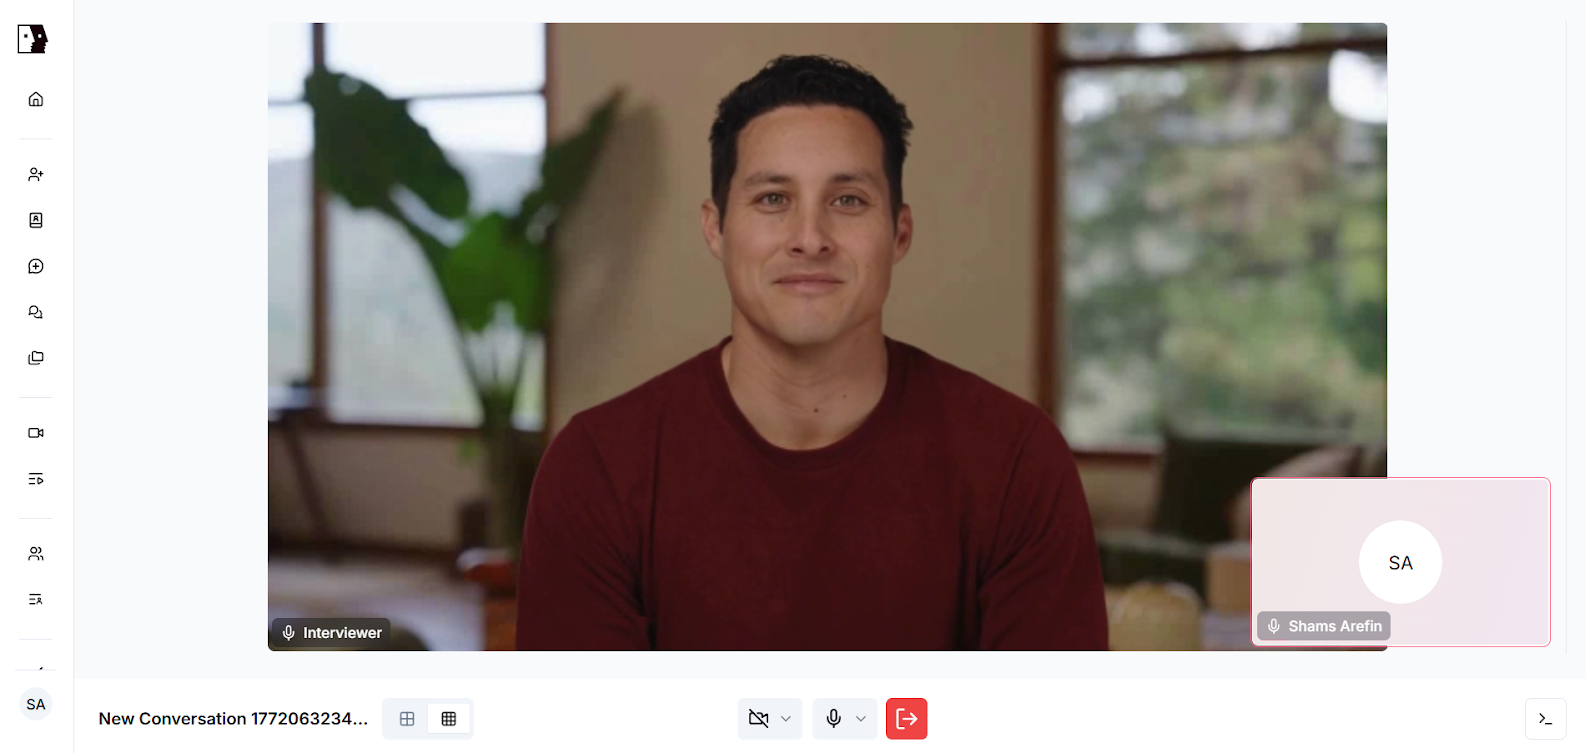
\includegraphics[width=0.8\textwidth]{Tavus.png}
    \caption{Tavus Interface}
    \label{fig: Tavus Interface}
\end{figure}


\item
\textbf{EMO (2024) : }EMO \cite{tian2024emo} generates expressive portrait animation from audio with a 2D diffusion model. It gives very expressive results, but at high computational cost and without real-time operation. Our system trades some expressiveness, since it animates the mouth region only, for real-time rendering on a laptop.\\

\begin{figure}[H]
    \centering
    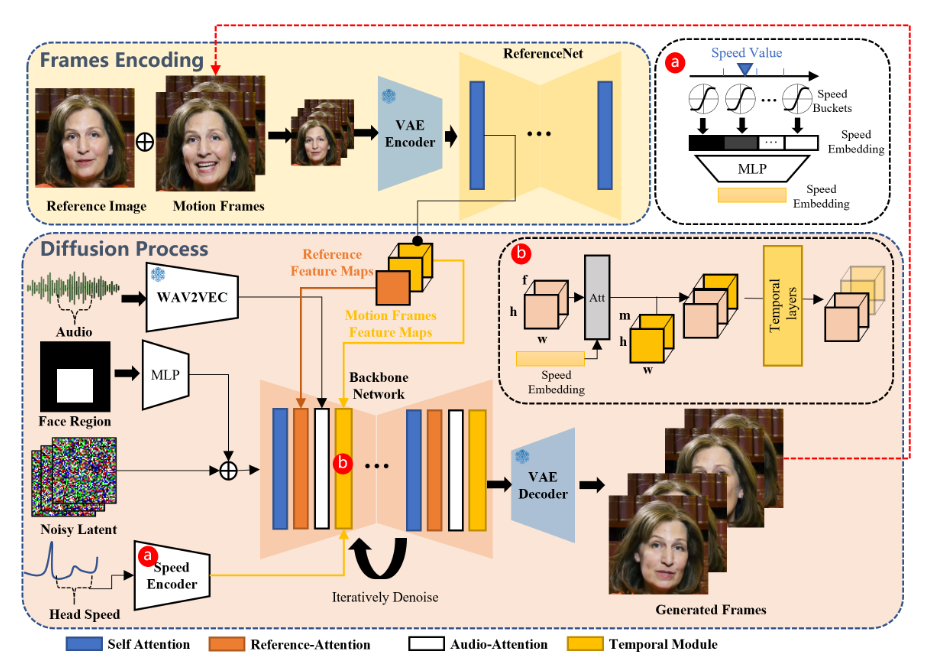
\includegraphics[width=0.8\textwidth]{EMO.png}
    \caption{EMO Methodology}
    \label{fig: EMO Methodology}
\end{figure}


\item
\textbf{SadTalker (2023) : }SadTalker \cite{zhang2023sadtalker} predicts 3D morphable-model parameters from audio and re-renders the face with a neural renderer. It is widely used but suffers from identity drift, unstable eye regions and jittery motion. Because our system edits only the mouth of a real recording of the speaker, the speaker's identity, eyes and head motion come directly from real video.\\

\begin{figure}[H]
    \centering
    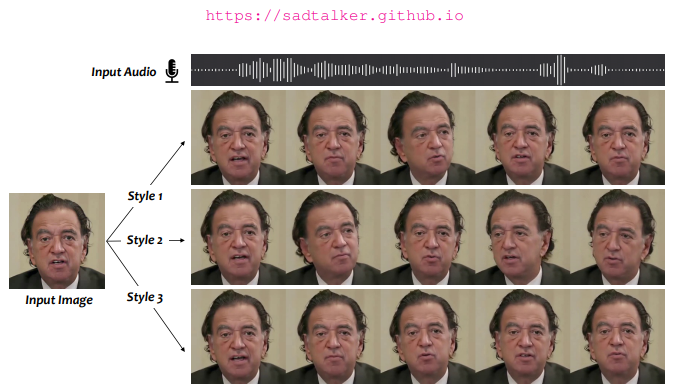
\includegraphics[width=0.8\textwidth]{SadTalker.png}
    \caption{SadTalker}
    \label{fig: SadTalker}
\end{figure}



\item
\textbf{InsTaG (CVPR 2025) : }InsTaG \cite{li2025instaglearningpersonalized3d} is a 3D Gaussian Splatting talking head that combines a universal motion field with a dynamic deformation network, giving strong identity preservation and stable motion. It is trained on English audio. We initially considered InsTaG for this project, but chose a 2D model because our requirement was real-time rendering on a 4~GB laptop GPU.\\

\begin{figure}[H]
    \centering
    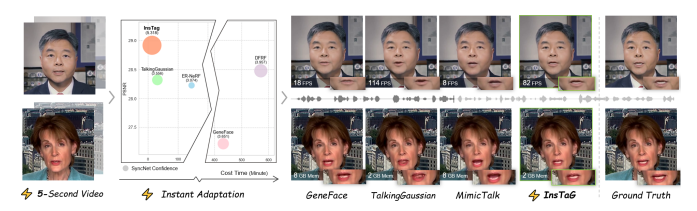
\includegraphics[width=0.8\textwidth]{InsTag.png}
    \caption{InsTaG Methodology}
    \label{fig: InsTag Methodology}
\end{figure}



\item
\textbf{Wav2Lip and SyncNet-based systems : }Wav2Lip \cite{prajwal2020wav2lip} generates the mouth in 2D and is known for strong lip-sync scores. We found that those scores need care: on our Bangla clip and on the public HDTF dataset, Wav2Lip scores \textit{above real video} of the same speaker on the standard lip-sync metric (Section~\ref{sec:leakage}), because it was trained against the same SyncNet that grades it.\\

\begin{figure}[H]
    \centering
    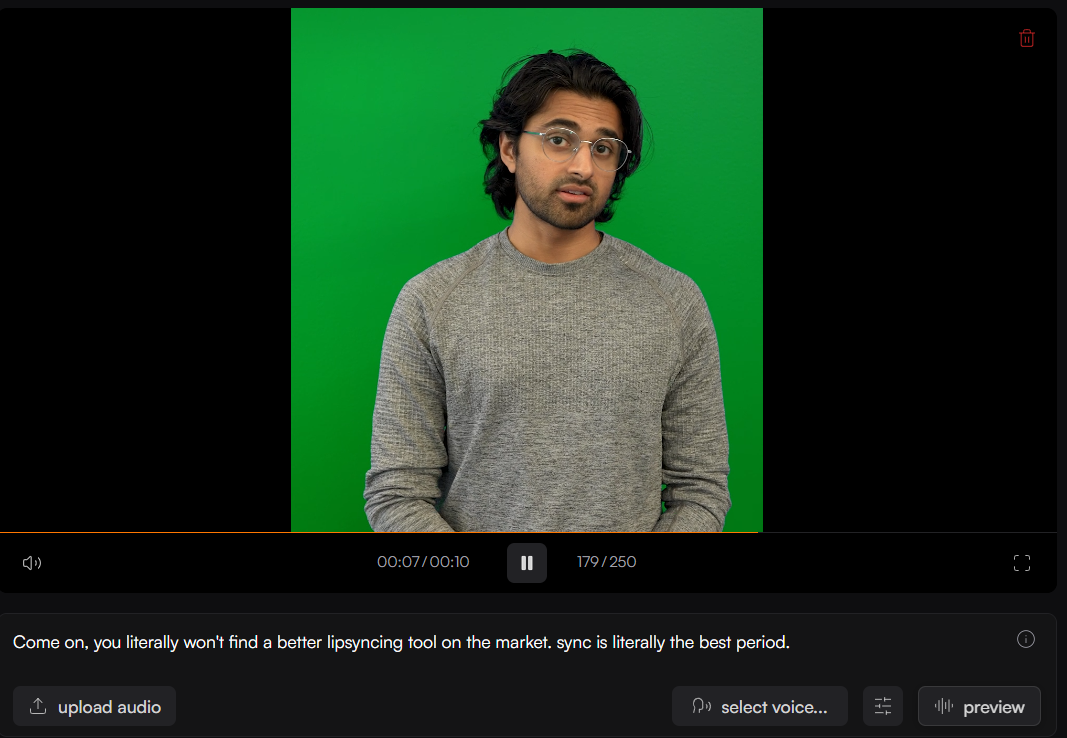
\includegraphics[width=0.8\textwidth]{Wav2Lip.png}
    \caption{Wav2Lip Interface}
    \label{fig: Wav2Lip Interface}
\end{figure}



\item
\textbf{NeRF-based head avatars : }Models such as AD-NeRF \cite{DBLP:journals/corr/abs-2103-11078} give high-quality reenactment but need long training and struggle with head poses outside the training data. Gaussian Splatting models render faster, but still need more GPU than a consumer laptop provides.\\

\end{enumerate}



\section{Gap Analysis}

\begin{table}[H]
\centering
\caption{Comparison of existing talking-head synthesis methods with the proposed system}
\label{tab:comparison}
\renewcommand{\arraystretch}{1.3}

\adjustbox{max width=\textwidth}{
\begin{tabular}{|p{4.2cm}|c|c|c|c|c|c|}
\hline
\textbf{Paper}
& \textbf{SyncTalk}
& \textbf{GaussianTalker}
& \textbf{InsTaG}
& \textbf{TalkingGaussian}
& \textbf{NeRFFaceSpeech}
& \textbf{Alapon (ours)} \\
\hline

Speech-driven talking head generation
& \cmark & \cmark & \cmark & \cmark & \cmark & \cmark \\
\hline

Trained and evaluated on Bangla speech
& \xmark & \xmark & \xmark & \xmark & \xmark & \cmark \\
\hline

Bangla-trained lip-sync expert
& \xmark & \xmark & \xmark & \xmark & \xmark & \cmark \\
\hline

Bangla audio-visual dataset
& \xmark & \xmark & \xmark & \xmark & \xmark & \cmark \\
\hline

Real-time shown on a laptop GPU$^{*}$
& \xmark & \xmark & \xmark & \xmark & \xmark & \cmark \\
\hline

Silent-audio leakage test reported$^{*}$
& \xmark & \xmark & \xmark & \xmark & \xmark & \cmark \\
\hline

Phoneme-level (viseme) supervision
& \xmark & \xmark & \xmark & \xmark & \xmark & partial$^{\dagger}$ \\
\hline

\end{tabular}
}

\vspace{0.3em}
{\footnotesize $^{*}$As reported in the original publications, which evaluate on desktop or datacentre GPUs. $^{\dagger}$A Bangla phoneme-to-viseme mapping is defined and used for evaluation; using it as a training signal is future work.}
\end{table}

\noindent
Current talking-head systems achieve speech-driven animation with high visual quality, but none of those in Table~\ref{tab:comparison} is trained or evaluated on Bangla, and none reports whether its mouth stays still when the audio is silent, the simplest test that the mouth is actually driven by the audio. Most also require GPUs well beyond consumer hardware. The proposed system addresses these gaps with Bangla training data, a Bangla-trained lip-sync expert, a silent-audio leakage test, and a model small enough to run in real time on a laptop. Phoneme-level lip-shape supervision is only partly addressed and is identified as future work.

\section{Summary}
Current talking-head systems such as SyncTalk, InsTaG, GaussianTalker and NeRFFaceSpeech have made major advances in high-quality audio-driven facial synthesis using NeRF and 3D Gaussian Splatting, reaching impressive realism and, in some cases, real-time rendering on powerful GPUs. 2D lip-synchronisation methods such as Wav2Lip, MuseTalk and LatentSync are widely used for dubbing. Almost all of them, however, are developed and evaluated on high-resource languages, and rarely check whether their mouth motion is truly driven by the audio. This motivates a real-time Bangla speech-driven avatar that is trained on Bangla data, verified to be driven by the audio rather than by the input video, and light enough to run on consumer hardware.\\
